\documentclass{article}

\usepackage{fancyhdr}
\usepackage{extramarks}
\usepackage{amsmath}
\usepackage{amsthm}
\usepackage{amsfonts}
\usepackage{tikz}
\usepackage[plain]{algorithm}
\usepackage{algpseudocode}

\usetikzlibrary{automata,positioning}

%
% Basic Document Settings
%

\usepackage{graphicx, url}
\graphicspath{figures/}

\topmargin=-0.45in
\evensidemargin=0in
\oddsidemargin=0in
\textwidth=6.5in
\textheight=9.0in
\headsep=0.25in

\linespread{1.1}

\pagestyle{fancy}
\lhead{\hmwkAuthorName}
\chead{\hmwkClass}
\rhead{\hmwkTitle}
\lfoot{\lastxmark}
\cfoot{\thepage}

\renewcommand\headrulewidth{0.4pt}
\renewcommand\footrulewidth{0.4pt}

\setlength\parindent{0pt}

%
% Create Problem Sections
%

\newcommand{\enterProblemHeader}[1]{
    \nobreak\extramarks{}{Problem \arabic{#1} continued on next page\ldots}\nobreak{}
    \nobreak\extramarks{Problem \arabic{#1} (continued)}{Problem \arabic{#1} continued on next page\ldots}\nobreak{}
}

\newcommand{\exitProblemHeader}[1]{
    \nobreak\extramarks{Problem \arabic{#1} (continued)}{Problem \arabic{#1} continued on next page\ldots}\nobreak{}
    \stepcounter{#1}
    \nobreak\extramarks{Problem \arabic{#1}}{}\nobreak{}
}

\setcounter{secnumdepth}{0}
\newcounter{partCounter}
\newcounter{homeworkProblemCounter}
\setcounter{homeworkProblemCounter}{1}
\nobreak\extramarks{Problem \arabic{homeworkProblemCounter}}{}\nobreak{}

%
% Homework Problem Environment
%
% This environment takes an optional argument. When given, it will adjust the
% problem counter. This is useful for when the problems given for your
% assignment aren't sequential. See the last 3 problems of this template for an
% example.
%
\newenvironment{homeworkProblem}[1][-1]{
    \ifnum#1>0
        \setcounter{homeworkProblemCounter}{#1}
    \fi
    \section{Problem \arabic{homeworkProblemCounter}}
    \setcounter{partCounter}{1}
    \enterProblemHeader{homeworkProblemCounter}
}{
    \exitProblemHeader{homeworkProblemCounter}
}

%
% Homework Details
%   - Title
%   - Due date
%   - Class
%   - Section/Time
%   - Instructor
%   - Author
%

\newcommand{\hmwkTitle}{Homework\ \#1}
\newcommand{\hmwkDueDate}{January 23, 2019}
\newcommand{\hmwkClass}{AMATH 515 (Optimization)}
\newcommand{\hmwkClassTime}{Section A}
\newcommand{\hmwkClassInstructor}{Prof. Alexander Aravkin}
\newcommand{\hmwkAuthorName}{\textbf{Alexey Sholokhov}}

%
% Title Page
%

\title{
    \vspace{2in}
    \textmd{\textbf{\hmwkClass:\ \hmwkTitle}}\\
    \normalsize\vspace{0.1in}\small{Due\ on\ \hmwkDueDate\ at 23:59}\\
    \vspace{0.1in}\large{\textit{\hmwkClassInstructor\ \hmwkClassTime}}
    \vspace{3in}
}

\author{\hmwkAuthorName}
\date{}

\renewcommand{\part}[1]{\textbf{\large Part \Alph{partCounter}}\stepcounter{partCounter}\\}

%
% Various Helper Commands
%

% Useful for algorithms
\newcommand{\alg}[1]{\textsc{\bfseries \footnotesize #1}}

% For derivatives
\newcommand{\deriv}[1]{\frac{\mathrm{d}}{\mathrm{d}x} (#1)}

% For partial derivatives
\newcommand{\pderiv}[2]{\frac{\partial}{\partial #1} (#2)}

% Integral dx
\newcommand{\dx}{\mathrm{d}x}

% Alias for the Solution section header
\newcommand{\solution}{\textbf{\large Solution}}

% Probability commands: Expectation, Variance, Covariance, Bias
\newcommand{\Var}{\mathrm{Var}}
\newcommand{\Cov}{\mathrm{Cov}}
\newcommand{\Bias}{\mathrm{Bias}}
\DeclareMathOperator{\dom}{Dom}
\DeclareMathOperator{\diag}{Diag}

%% \mathbb symbols
\DeclareMathOperator{\E}{\mathbb{E}}
\DeclareMathOperator{\A}{\mathbb{A}}
\DeclareMathOperator{\R}{\mathbb{R}}
\DeclareMathOperator{\X}{\mathbb{X}}
\DeclareMathOperator{\N}{\mathbb{N}}
\DeclareMathOperator{\Q}{\mathbb{Q}}

%% \mathcal symbols
\DeclareMathOperator{\RR}{\mathcal{R}}
\DeclareMathOperator{\PP}{\mathcal{P}}
\DeclareMathOperator{\NN}{\mathcal{N}}
\DeclareMathOperator{\CC}{\mathcal{C}}

%% Q.E.D. 

\begin{document}

\maketitle

\pagebreak

    \textbf{Notation}: For this assignment let $x_1, x_2 \in \dom(f)$, and let $x = \lambda x_1 + (1 - \lambda) x_2$ for some $\lambda \in [0, 1]$, where $f$ is a function from the problem we work on. 

\begin{homeworkProblem}
    Explain why each of the following functions is convex:
    \begin{enumerate}
        \item[a)] \( \delta_C (x) = \begin{cases} 
            0, &  x \in C \\
            \infty,  & x \not \in C  
        \end{cases} \), $\quad C$ is convex
        \item[b)] \(\sigma_C (x) = \sup_{c \in C} c^Tx \)
        \item[c)] \(f(x, t) = tg(x/t)\) where $g$ is a convex function, $x \in \R^n$
    \end{enumerate}
    
    \textbf{Solution}
        
    \begin{itemize}
        \item[a)] Let $x_1, x_2 \in C$, so $x \in C$, as $C$ is convex. Then $\delta_C(x) = 0 \leq 0 = \lambda \delta_C(x_1) + (1 - \lambda)\delta_C(x_2)$. 
        If either $x_1 \not \in C$ or $x_2 \not \in C$ then $\lambda \delta_C (x_1) + (1 - \lambda)\delta_C(x_2) = \infty \geq \delta_C(x)$ whatever $x$ is by the definition of infinity. 
        \item[b)] \(\sigma_C(x) = \sigma_C(\lambda x_1 + (1 - \lambda) x_2) = \sup_{c \in C}c^T(\lambda x_1 + (1 - \lambda) x_2) \leq \lambda\sup_{c \in C} c^Tx_1 + (1 - \lambda)\sup_{c \in C} c^Tx_2 = \lambda \sigma_C(x_1) + (1 - \lambda)\sigma_C(x_2)\) 
        \item[c)] For any $(x_1, t_1), (x_2, t_2) \in \R\times\R_+$ \\ \(f(x, t) = (\lambda t_1 + (1-\lambda)t_2)g\left( \frac{\lambda x_1 + (1-\lambda)x_2}{\lambda t_1 + (1 - \lambda) t_2}\right) = (\lambda t_1 + (1-\lambda)t_2)g\left(\frac{(1 - \lambda)t_1}{(1-\lambda)t_1+\lambda t_2}\frac{x_1}{t_1} + \frac{\lambda t_2}{(1-\lambda)t_1+\lambda t_2}\frac{x_2}{t_2} \right) \leq (1-\lambda) t_1 g\left(\frac{x_1}{t_1}\right) + \ t_1 g\left(\frac{x_1}{t_1}\right)\)
    \end{itemize}    

\end{homeworkProblem}


\begin{homeworkProblem}
Let $f, g \in \CC^2(\R),\, h = f(g(x))$
\begin{enumerate}
    \item[a)] Let $f$ and $g$ be convex. Is $h$ convex?
    \item[b)] Let $f$ be convex and $g$ be concave. Is $h$ convex? 
    \item[c)] Let $f$ be convex and $g$ be affine. Prove that $h$ is convex.
    \item[d)] Show that the following functions are convex: 
        \begin{enumerate}
            \item[i)] Logistic regression objective: \(\sum_{i = 1}^n \log(1 + e^{a_i^Tx}) - b^TAx\)
            \item[ii)] Poisson regression objective: \(\sum_{i = 1}^n e^{a^T_ix} - b^TAx\)
        \end{enumerate}    
\end{enumerate}

\textbf{Solution}
\begin{enumerate}
    \item[a)] $h$ is not convex. \textbf{A counter example}: \(f(x) = x^{-1} \text{ -- convex}, \, g(x) = -x \text{ -- convex} \implies h(x) = -x^{-1}\) which is concave.
        Recalling the convexity criterion from calculus to provide a sufficient condition: 
        \begin{equation}
        \label{eq:convexity_criterion}
            f(x) \text{ is convex in} \R \quad \iff \quad \forall x \in \R \, f''(x) \geq 0             
        \end{equation}
        \[h'(x) = f'\left(g(x)\right)g'(x)\]
        \[h''(x) = \underbrace{f''(g(x))}_{\geq 0 \text{ as f is convex}}\underbrace{\left(g'(x)\right)^2}_{\geq 0} + f'(x)\underbrace{g''(x)}_{\geq 0 \text{ as g is convex}}\]
        So we need $f'(x) \geq 0$ which means that \textbf{$f$ should be non-decreasing}. \qed
    \item[b)] $h$ is not convex. \textbf{A counter example:} \(f = x^{\frac{3}{2}} \text{ is convex},\, g = \sqrt{x} \text{ is concave, but } h = x^{\frac{3}{4}}\) is concave. 
    We use the same criterion: 
    \[h''(x) = \underbrace{f''(g(x))}_{\geq 0 \text{ as f -- convex}}\underbrace{\left(g'(x)\right)^2}_{\geq 0} + f'(x)\underbrace{g''(x)}_{\leq 0 \text{ as g -- concave}}\]
    So we need $f'(x) \leq 0$ which means that \textbf{$f$ should be non-increasing}. \qed
    \item[c)] Let $g(x) = Ax + b$ be affine. So \(h(x) = f(g(x)) = f(Ax + b) = f(\lambda Ax_1 + (1 - \lambda)Ax_2 + \lambda b + (1 - \lambda)b) \leq \)
    \\
    \(\leq \lambda f(Ax_1 + b) + (1 - \lambda)f(Ax_2 + b) = \lambda h(x_1) + (1-\lambda)h(x_2)\) \qed
    \item[d)]
    \begin{enumerate}
        \item[i)] First, note that \(g(x) = \log(1 + e^x)\) is convex due to the convexity criterion $\frac{\partial^2}{\partial x^2}g(x) = \frac{e^x}{(1 + e^-x)^2} \geq 0$. $h(x) = a_i^Tx$ is affine. Hence, $f(x) = g(h(x)) = \log(1 + e^{a_i^Tx})$ is convex due to (c). 
        
            Next, $-b^TAx$ is a linear function of $x$, so it is convex. And, finally, a sum over $n+1$ convex functions is convex. \qed
        \item[ii)] $e^x$ is a convex function, as $\frac{d^2}{dx^2}e^x = e^x \geq 0$. $h(x) = a_i^Tx$ is affine. Hence $e^{a_i^Tx}$ is convex due to (c). Finally, the sum of $n$ convex functions and one linear function is convex. \qed 
    \end{enumerate} 
\end{enumerate}
 

\end{homeworkProblem}

\begin{homeworkProblem}
A function is strictly convex if 
\[
    f(\lambda x_1 + (1 - \lambda)x_2) < \lambda f(x_1) + (1 - \lambda)f(x_2)
\]
$\lambda \in (0,1)$.
\begin{enumerate}
    \item[a)] Give an example of a strictly convex function which does not have a minimizer.
    \item[b)] Show that a sum of a strictly convex function and a convex function is strictly convex.
    \item[c)] What conditions (if any) are necessary to ensure that the following problems have a unique minimizer?
    \begin{enumerate}
        \item[i)] \(\min_x \frac{1}{2}\|Ax - b\|^2\)
        \item[ii)] \(\min_x \sum_{i = 1}^n \log(1 + e^{a_i^Tx}) - b^TAx\)
        \item[iii)] \(\min_x \sum_{i = 1}^n \log(1 + e^{a_i^Tx}) - b^TAx + \lambda(\alpha\|x\|_1 + (1 - \alpha)\|x\|^2), \quad \lambda > 0, \, \alpha > 0\)
    \end{enumerate}
\end{enumerate}

\textbf{Solution}
The strict convexity criterion from the Boyd's book "Convex Optimization" will be used:

\[
    f(x) \text{ is strictly convex} \iff \|\nabla^2f(x)\| > 0 \text{ everywhere}
\]

\begin{enumerate}
    \item[a)] An example is \(f(x) = e^x\) as \(\frac{d^2}{dx^2}e^x = e^x > 0\) everywhere, yet \(\arg \min_x e^x = - \infty\) \qed
    \item[b)] Let $f$ be convex and $g$ be strictly convex.
    
    \(f(x) + g(x) = f(\lambda x_1 + (1 - \lambda)x_2) + g(\lambda x_1 + (1 - \lambda)x_2) < f(\lambda x_1 + (1 - \lambda)x_2) + \lambda g(x_1) + (1 - \lambda)g(x_2) \leq \)
    \\
    \(\leq \lambda(f(x_1) + g(x_1)) + (1 - \lambda)(f(x_2) + g(x_2))\) \qed
    \item[c)] For (i) and (ii) the second order necessary conditions (Theorem 2.8 in the course book) will be used: 
    \[
        \text{If } x \in U \text{ is a local minimizer, then } \nabla f(x) = 0 \text{ and } \nabla^2 f(x) \succeq 0
    \] 
    \begin{enumerate}
        \item[i)] \(\nabla f(x) = A^T(Ax - b) = 0 \implies A^TAx = A^Tb \) -- the normal equation should hold.
        Also, \(\nabla^2 f(x) = A^TA \succeq 0\) for all $x$ as \(x^TA^TAx = (Ax)^TAx = \|Ax\| \geq 0\) for all $x$, so this condition always holds. \qed
        \item[ii)] \(\nabla f(x) = A^T\sigma(Ax) - A^Tb\) where $\sigma(y) = \frac{1}{1+e^{-y}}$, and $\sigma(x) \in \R^n \text{ for } x \in \R^n$ means the vectorized form (element wise application). So we need to ensure that $\sigma(Ax) - b \in Ker(A)$. Also, note that \( \nabla^2f(x) = A^T\diag(\sigma(Ax)\sigma(-Ax))A \succeq 0\) for all $x$: let $M = \sqrt{\diag(\sigma(Ax)\sigma(-Ax))}$ (all the diagonal elements are positive for all $x$), then we have: \(y^TA^T\diag(\sigma(Ax)\sigma(-Ax))Ay = y^TA^TM^TMAy = \|MAy\| = \|Ay\|_{M^TM} \geq 0 \) for all $y \in \R^n$, so the Hessian condition always holds. \qed
        \item[iii)] This function is strictly convex as a sum of a strictly convex function ($\frac{\lambda}{2}\|x\|^2$) and convex ones (see 3b), so the minimizer is unique, if exists. The function is non-differentiable yet continuous. Hence, due to the Weierstrass Theorem, it is enough to ensure that the domain of the function is finite and convex to guarantee the existence of a unique minimizer.\qed
    \end{enumerate}
\end{enumerate}
\end{homeworkProblem}

\begin{homeworkProblem}

Find the global bound for $\beta$ (if any) for the following objectives: 
\begin{enumerate}
    \item[a)] \(\frac{1}{2}\|Ax - b\|^2\)
    \item[b)] \(\sum_{i = 1}^n \log(1 + e^{a^T_ix}) + \frac{\lambda}{2}\|x\|^2 \)
    \item[c)] \(\sum_{i = 1}^n e^{a^T_ix} - b^TAx\)
\end{enumerate}

\textbf{Solution}
For (a) and (b) I'll use the Theorem 1 from the lecture notes: 
    \[ f \in \CC_\beta^{2, 1} \iff \forall x\: \| \nabla^2f(x)\| \leq \beta \]
    
    \begin{enumerate}
        \item[a)] $\|\nabla^2 f(x)\| = \|A^TA\| = \sigma_1(A^TA) = \beta$ where $\sigma_1(X)$ is the largest singular value for the matrix $X$. \qed
        \item[b)] $\|\nabla^2 f(x)\| = \|A^T\diag(\sigma(Ax)\sigma(-Ax))A + \lambda I\|  \leq \frac{1}{4}\|A^TA\|\|\diag(\sigma(Ax)\sigma(-Ax))\| + \lambda \leq \frac{1}{4}\sigma_1(A^TA)\max(\sigma(Ax)) + \lambda$ \qed
        \item[c)] There is no $\beta$ for this function. Let's prove it as contra positive: suppose there is $\beta$ such that for any $x$ and $y$
        \[
            \|\nabla f(x) - \nabla f(y)\| \leq \beta\|x - y\|
        \]
        holds. Let $y = 0$ and $x_\alpha = \alpha e_i$ such that $e^{a_i} \not \in \ker(A)$. Such $i$ always exists if $A \not = 0^{m \times n}$ So 
        \[
            \|\sum_{j = 1}^n a_j(e^{\alpha A_{ij}} - 1) \| = \|Ae^{\alpha a_i}\| \leq \beta\alpha
        \]
        
        Easy to see that $\lim_{\alpha \to \infty} \frac{Ae^{\alpha a_i}}{\alpha} = \infty > \beta$, which concludes the proof. \qed
        
    \end{enumerate}
\end{homeworkProblem}

\begin{homeworkProblem}
    \begin{enumerate}
        \item[a)]
        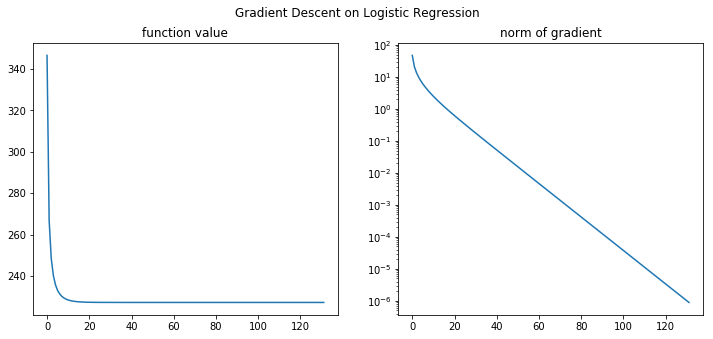
\includegraphics[width=0.9\textwidth]{figures/grad_lgt}
        \item[b)]
        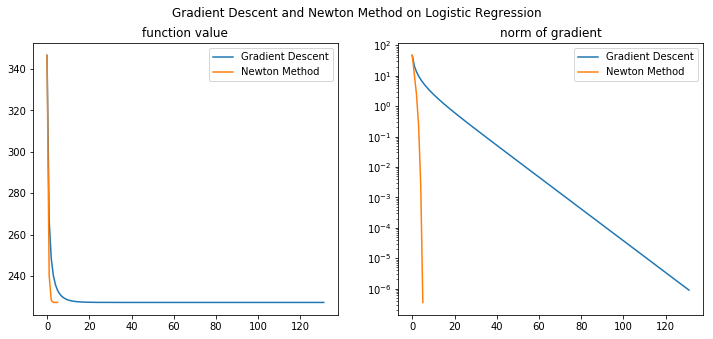
\includegraphics[width=0.9\textwidth]{figures/grad_newton_lgt}
        
        Both methods converge, yet the Newton method converges 20 times faster than the Gradient Descent. 
        \item[c)] 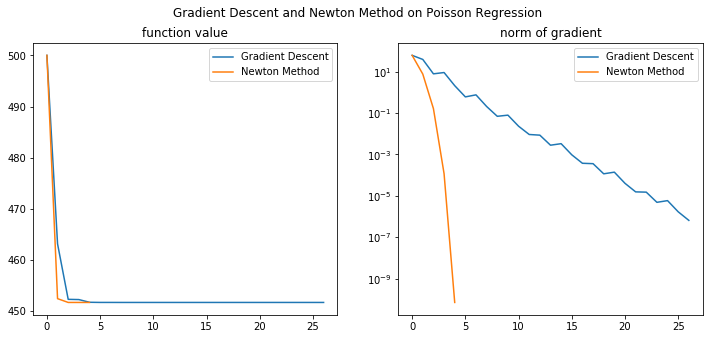
\includegraphics[width=0.9\textwidth]{figures/grad_newton_poisson}
        \item[d)] Newton Method converges with acceleration over time, while the Gradient Descent method converges with a fixed rate in terms of a logarithmic plot. It illustrates the theoretical result that the Newton Method converges quadratically while the Gradient Descent algorithm converges linearly. Also, it means that the starting point was pretty close to the solution, as the fixed step-size Newton method converges. 
    \end{enumerate}
\end{homeworkProblem}

\end{document}
